\documentclass[12pt,]{article}
\usepackage{lmodern}
\usepackage{amssymb,amsmath}
\usepackage{ifxetex,ifluatex}
\usepackage{fixltx2e} % provides \textsubscript
\ifnum 0\ifxetex 1\fi\ifluatex 1\fi=0 % if pdftex
  \usepackage[T1]{fontenc}
  \usepackage[utf8]{inputenc}
\else % if luatex or xelatex
  \ifxetex
    \usepackage{mathspec}
  \else
    \usepackage{fontspec}
  \fi
  \defaultfontfeatures{Ligatures=TeX,Scale=MatchLowercase}
\fi
% use upquote if available, for straight quotes in verbatim environments
\IfFileExists{upquote.sty}{\usepackage{upquote}}{}
% use microtype if available
\IfFileExists{microtype.sty}{%
\usepackage[]{microtype}
\UseMicrotypeSet[protrusion]{basicmath} % disable protrusion for tt fonts
}{}
\PassOptionsToPackage{hyphens}{url} % url is loaded by hyperref
\usepackage[unicode=true]{hyperref}
\hypersetup{
            pdftitle={Quantile Regression Analysis for Statin effects on glucose level},
            pdfborder={0 0 0},
            breaklinks=true}
\urlstyle{same}  % don't use monospace font for urls
\usepackage[margin=1in]{geometry}
\usepackage{longtable,booktabs}
% Fix footnotes in tables (requires footnote package)
\IfFileExists{footnote.sty}{\usepackage{footnote}\makesavenoteenv{long table}}{}
\usepackage{graphicx,grffile}
\makeatletter
\def\maxwidth{\ifdim\Gin@nat@width>\linewidth\linewidth\else\Gin@nat@width\fi}
\def\maxheight{\ifdim\Gin@nat@height>\textheight\textheight\else\Gin@nat@height\fi}
\makeatother
% Scale images if necessary, so that they will not overflow the page
% margins by default, and it is still possible to overwrite the defaults
% using explicit options in \includegraphics[width, height, ...]{}
\setkeys{Gin}{width=\maxwidth,height=\maxheight,keepaspectratio}
\setlength{\emergencystretch}{3em}  % prevent overfull lines
\providecommand{\tightlist}{%
  \setlength{\itemsep}{0pt}\setlength{\parskip}{0pt}}
\setcounter{secnumdepth}{5}
% Redefines (sub)paragraphs to behave more like sections
\ifx\paragraph\undefined\else
\let\oldparagraph\paragraph
\renewcommand{\paragraph}[1]{\oldparagraph{#1}\mbox{}}
\fi
\ifx\subparagraph\undefined\else
\let\oldsubparagraph\subparagraph
\renewcommand{\subparagraph}[1]{\oldsubparagraph{#1}\mbox{}}
\fi

% set default figure placement to htbp
\makeatletter
\def\fps@figure{htbp}
\makeatother

\usepackage{setspace}\doublespacing
\usepackage{float}

\title{Quantile Regression Analysis for Statin effects on glucose level}
\author{}
\date{\vspace{-2.5em}}

\begin{document}
\maketitle

{
\setcounter{tocdepth}{2}
\tableofcontents
}
\section{introduction}

Approximately, 18 million deaths annually per year are caused by
cardiovascular diseases(CVD) and similar to this number of nonfatal
cardiovascular events (Hay et al. 2017). For 2011, annual costs for CVD
and stroke were \(\$320.1\) billion, which is more than cancer cost.
This cost include \$195.6 billion in direct costs (healthcare costs),
and cost of future productivity loss is \$124.5 (Mozaffarian et al.
2015). Abnormal lipid ratio is a risk factor for CVD (Yusuf et al.
2004). Lowering low-density lipoprotein (LDL) using statin reduces risk
of cardiovascular diseases even with population with no CVD (Yusuf et
al. 2016). It is known that diabetes is a risk factor for CVD, however,
it is shown that elevated glucose, prediabetes,is also a risk factor for
CVD (Balkau et al. 2004).

Statin use associated with high risk of a new onset diabetes in
normoglcemic (HR 1.19,95\% CI , 1.05 to 1.35) and in prediabetes (HR
1.24 95\% CI , 1.11 to 1.38). On the other hand, overall mortality risks
went down in both normoglycemic (HR 0.70; 95 \% CI, 0.66 to 0.80) and
IFG patients (HR 0.77, 95 \% CI, 0.64 to 0.91) with statin use (Castro
et al. 2016). For population with one or more risk factor for diabetes,
statin use associate with 39\% reduction in the primary end points (the
hazard ratio (HR) 0.61), and a 28\% (HR 1.28)increase in diabetes(Ridker
et al. 2012).Pandya at el.{[}pandya2015{]} suggested the dis-utility
associated with taking a pill daily, statin price, and the risk of
statin-induced diabetes negatively impacted the cost effectiveness of
statin use recommendation.

Several studies esimated the association of different factors like waist
circumference, Cholestrol with the conditional mean of glucose using OLS
or logistic regression model. The drawback in these study is not
considering the dispersion of the association of covariates with
conditional distribution of the dependent variables, glucose levele.

\section{Quantile Regression}

Quantile regression is an important tool used to regress the dependent
variable with high variance over the independent variables. QR is
developed to study the relationships between variables that have week or
no-relationships between their means. One of the advantage of using QR
over OLS is robust for outliers.

For a random variable \(X\), the cumulative distribution function (CDF)
is \[F(X)=P(X\leq x)\], and the \(\tau\)th quantile of \(X\) is defined
by \[ F^{-1}(\tau)=\text{inf}\{x: F(x)\ge \tau\} \] where \(0<\tau<1\).
Let the loss function is defined by
\[\rho_{\tau}(u)= u(\tau-I_{(u<0)})\] where \(I\) is the indicator
function (Koenker 2005). The quantile estimator is the value that
minimizes the expected loss function

\(E\rho_{\tau}(X-\hat{x})=(\tau-1)\int_{-\infty}^{\hat{x}} (x-\hat{x})dF(x)+\tau\int_{\hat{x}}^{-\infty} (x-\hat{x})dF(x).\)
Differentiating with respect to \(\hat{x}\), we get
\[ 0  =(\tau-1)\int_{-\infty}^{\hat{x}} dF(x)+\tau\int_{\hat{x}}^{-\infty} dF(x)
=F(\hat{x})-\tau.\] Due to monotnicity of the cumulative distribution
function, any solution that satisfies \(\{x:F(x)=\tau \}\) is a
minimizing for the expected loss function.

Least square method expresses conditional mean of y given x as
\(\mu(x)=x^T\beta\) and it solves
\[ \underset{\beta\in \mathcal{R}^p}{\text{min}}\sum_{i=1}^n(y_i- x_i^T\beta)^2.\]
Quantile regression expresses conditional quantile function
\(Q_y(\tau|x)=x^T \beta ({\tau)}\) and solve
\[ \underset{\beta\in \mathcal{R}^p}{\text{min}}\sum_{i=1}^n\rho_{\tau}(y_i- x_i^T\beta)^2.\]This
minimization problem can be reformulated to a linear programming problem
\[ \underset{\beta\in \mathcal{R}^p}{\text{min}} \]

\subsection{Quantile Regression Technique }

\section{Methods}

A multivariate quantile regression model is used to assess the
characteristics of the association variability in different quantiles of
the conditional distribution of the glucose levels.

The dependent variables in our model are gender, race, age, BMI, total
cholesterol, Choesterol drug uses (yes or no), and waist circumference.
All type of cholesterol drug are included including statins. The
included races are non-Hispanic white, non-Hispanic black, Hispanic, or
other.

\section{Numerical Example}\subsection{Data}

The data used in this study is National Health and Nutrition Examination
Survey data (NHANES)(Disease Control and (CDC) 2018). The survey
examines a nationally representative sample of U.S. population.It
focuses on variety of health and nutrition measurements. In this study,
we cumulated 6 cycles of NHANES data (2007--2018). There are around
12,000 records. We selected population age between 20 and 80. BMI are
classified into different categories according to underweight, 18.5
kg/m2; normal weight, 18.5 to 25 kg/m2; overweight, 25 to 30 kg/m2;
obese, 30 to 35 kg/m2; and very obese more than 35 kg/m2.

\begin{longtable}[]{@{}lcr@{}}
\toprule
Syntax & Male & Femal\tabularnewline
\midrule
\endhead
count & 5990 & 6416\tabularnewline
Mean of Age & 49.9 & 49.73\tabularnewline
glucose & 112.618 & 106.47\tabularnewline
TC & Title & Here's this\tabularnewline
Statin use (ratio) & 0.198 & 0.181\tabularnewline
\bottomrule
\end{longtable}

\begin{figure}

{\centering 
\includegraphics[width=0.8\linewidth]{C:/Users/Muhannad/Desktop/multvariat/R_codes/tonton/BMI/images/exploratory} 

}

\caption{A better figure caption}\label{fig:data}
\end{figure}

to cite figure \#See Figure \ref{fig:data} However,.

\begin{figure}

{\centering 
\includegraphics[width=0.8\linewidth]{C:/Users/Muhannad/Desktop/multvariat/R_codes/tonton/BMI/images/exploratory2} 

}

\caption{A better figure caption}\label{fig:unnamed-chunk-1}
\end{figure}

So,

\begin{figure}

{\centering 
\includegraphics[width=0.8\linewidth]{C:/Users/Muhannad/Desktop/multvariat/R_codes/tonton/BMI/images/quant90} 

}

\caption{A better figure caption}\label{fig:unnamed-chunk-2}
\end{figure}\section{Results}

The resulting estimate of effects on conditional mean of glucose level
may not reflect the size and nature of theses effects on lower or upper
quantile. For example, in the Figure \ref{fig:resu1}, the conditional
mean shows the conditional mean effects of gender on glucose level is
about 7. However, the disparity of the gender effects on lower tails is
much smaller which is about 3 but the disparity is higher for the upper
tail of the distribution somewhat larger than 10 mg/dL.

From the OLS it is obvious statin users have on average higher glucose
levels if compared to non-statin users which is around 10 mg/dL. The
disparity in glucose level for statin users vs non-statin users is
negligible in the left tail, however, statin uses seems to be associated
with a rather large effects on glucose levels somewhat larger than 55
mg/dL for the right quantile.

\begin{figure}

{\centering 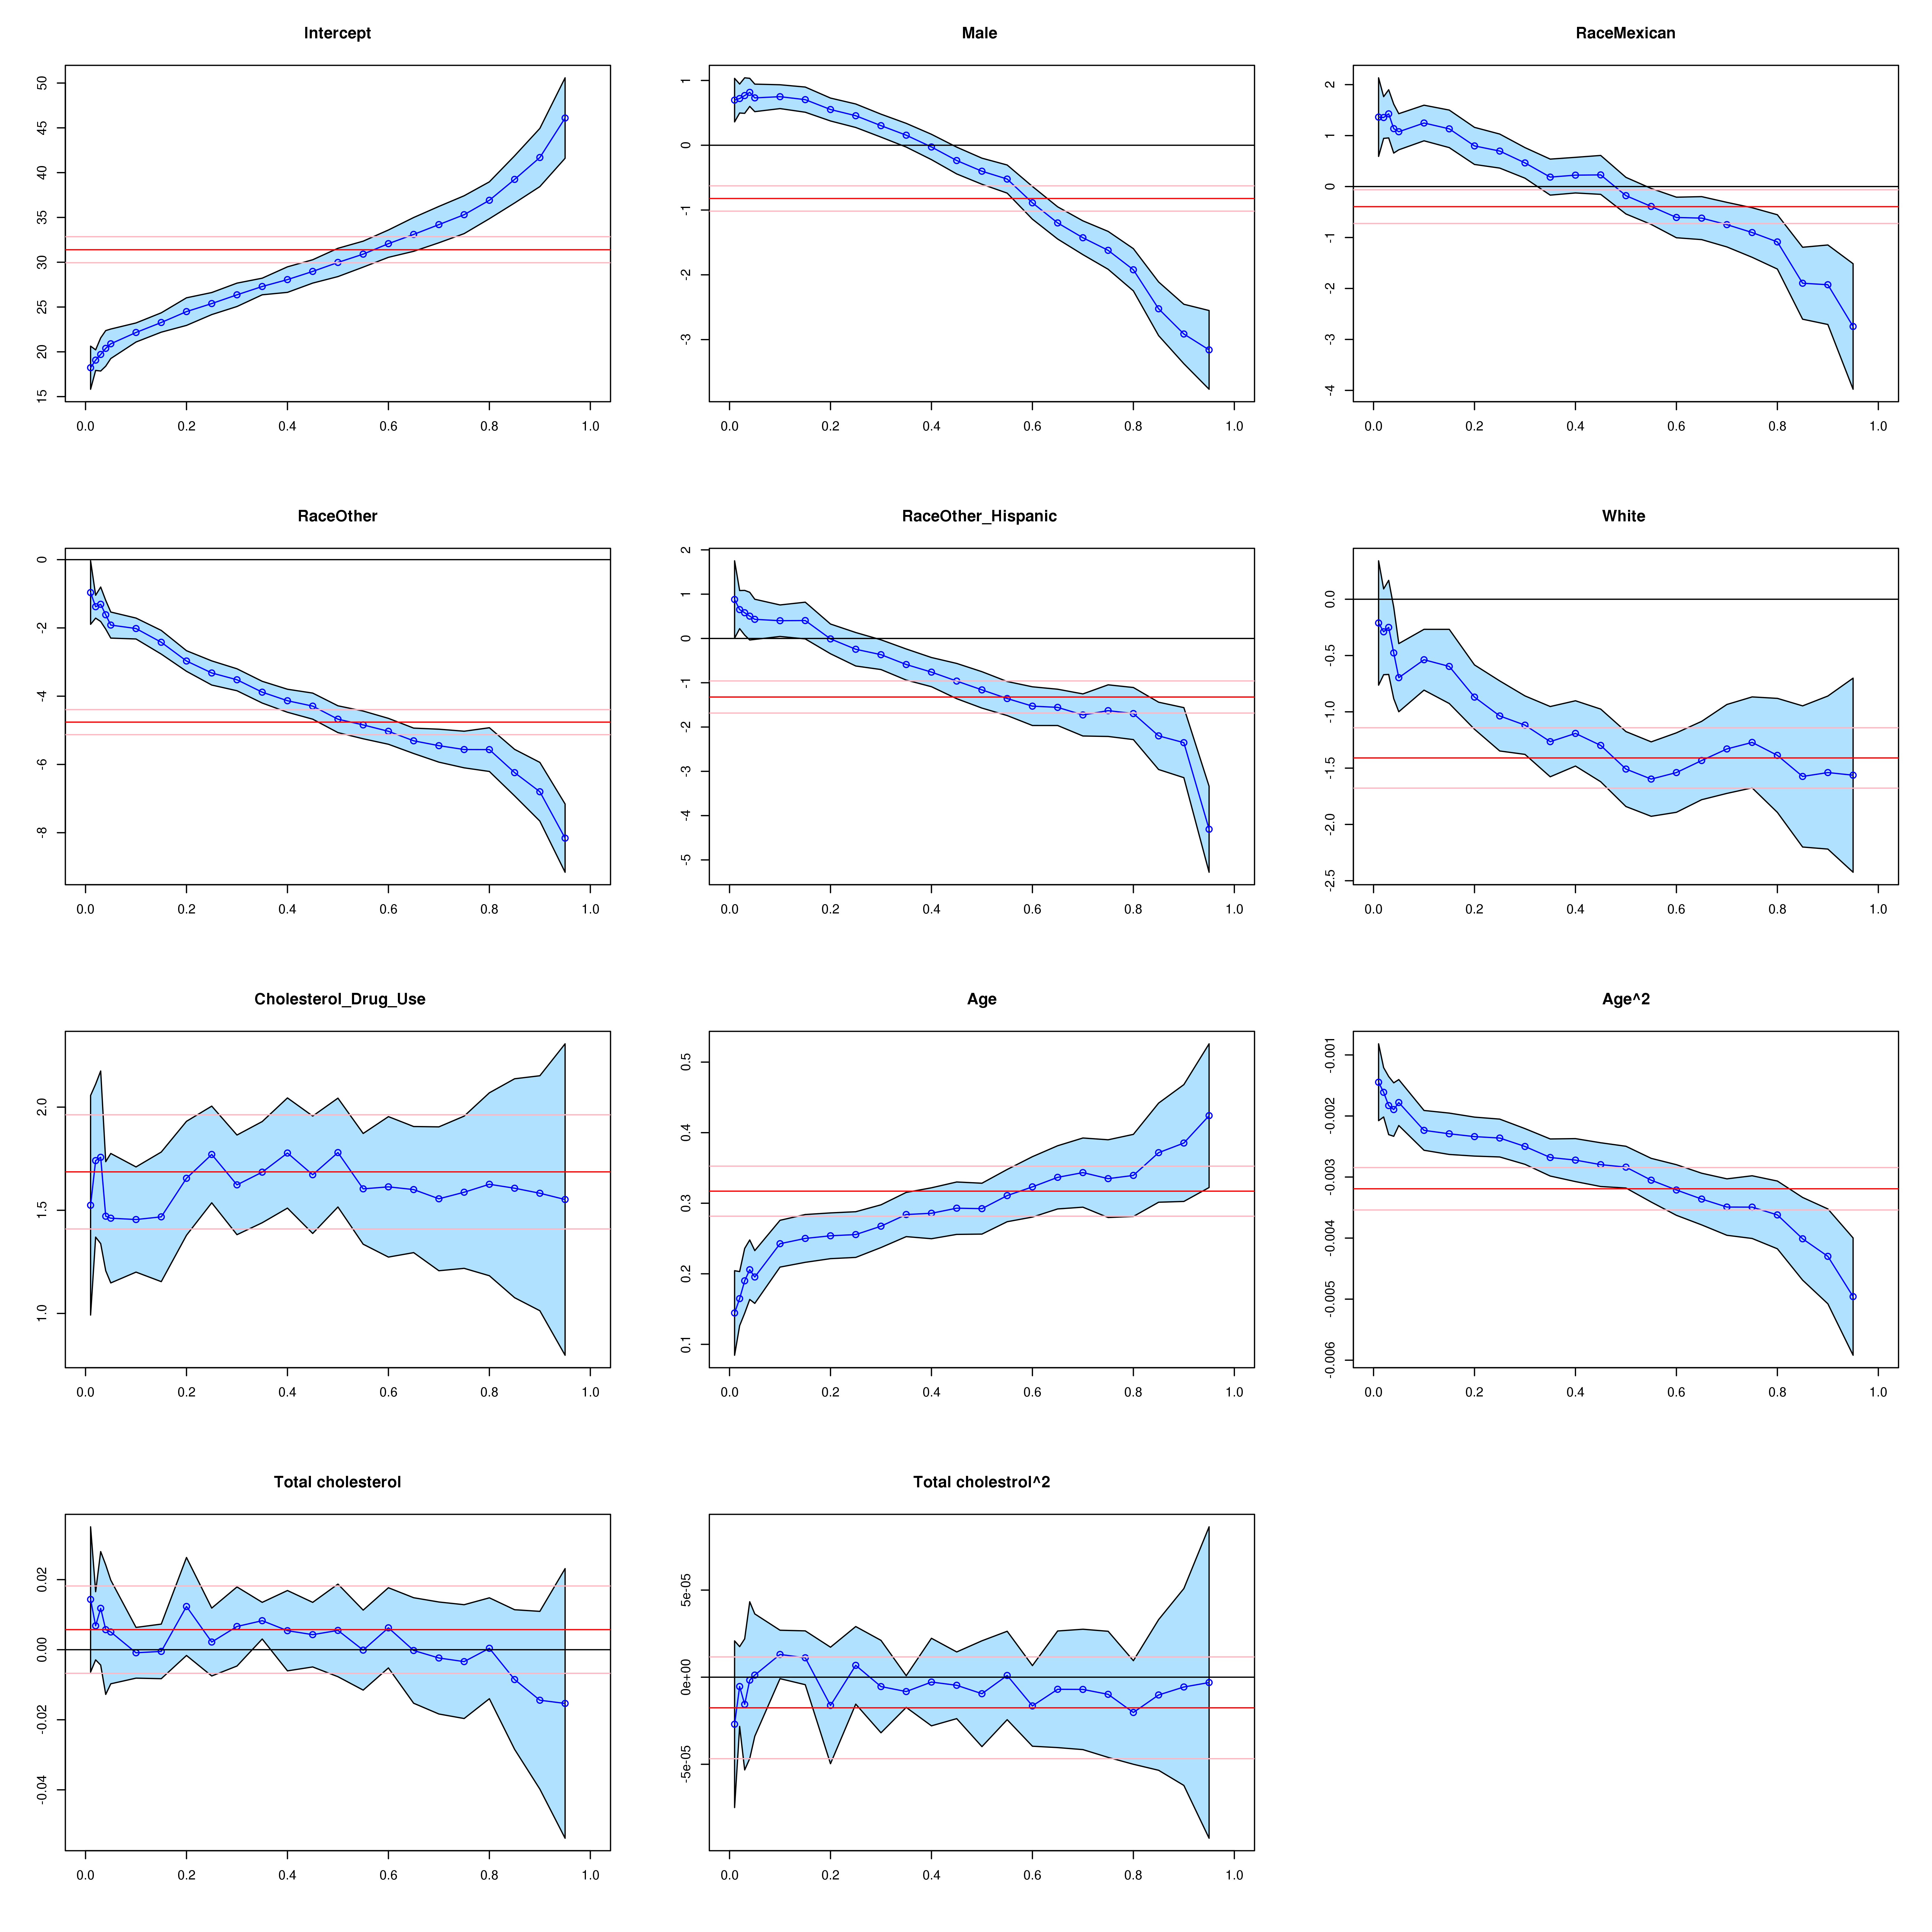
\includegraphics[width=0.8\linewidth]{C:/Users/Muhannad/Desktop/multvariat/R_codes/tonton/BMI/images/newfig} 

}

\caption{A better figure caption}\label{fig:resu1}
\end{figure}

So,

\begin{figure}

{\centering 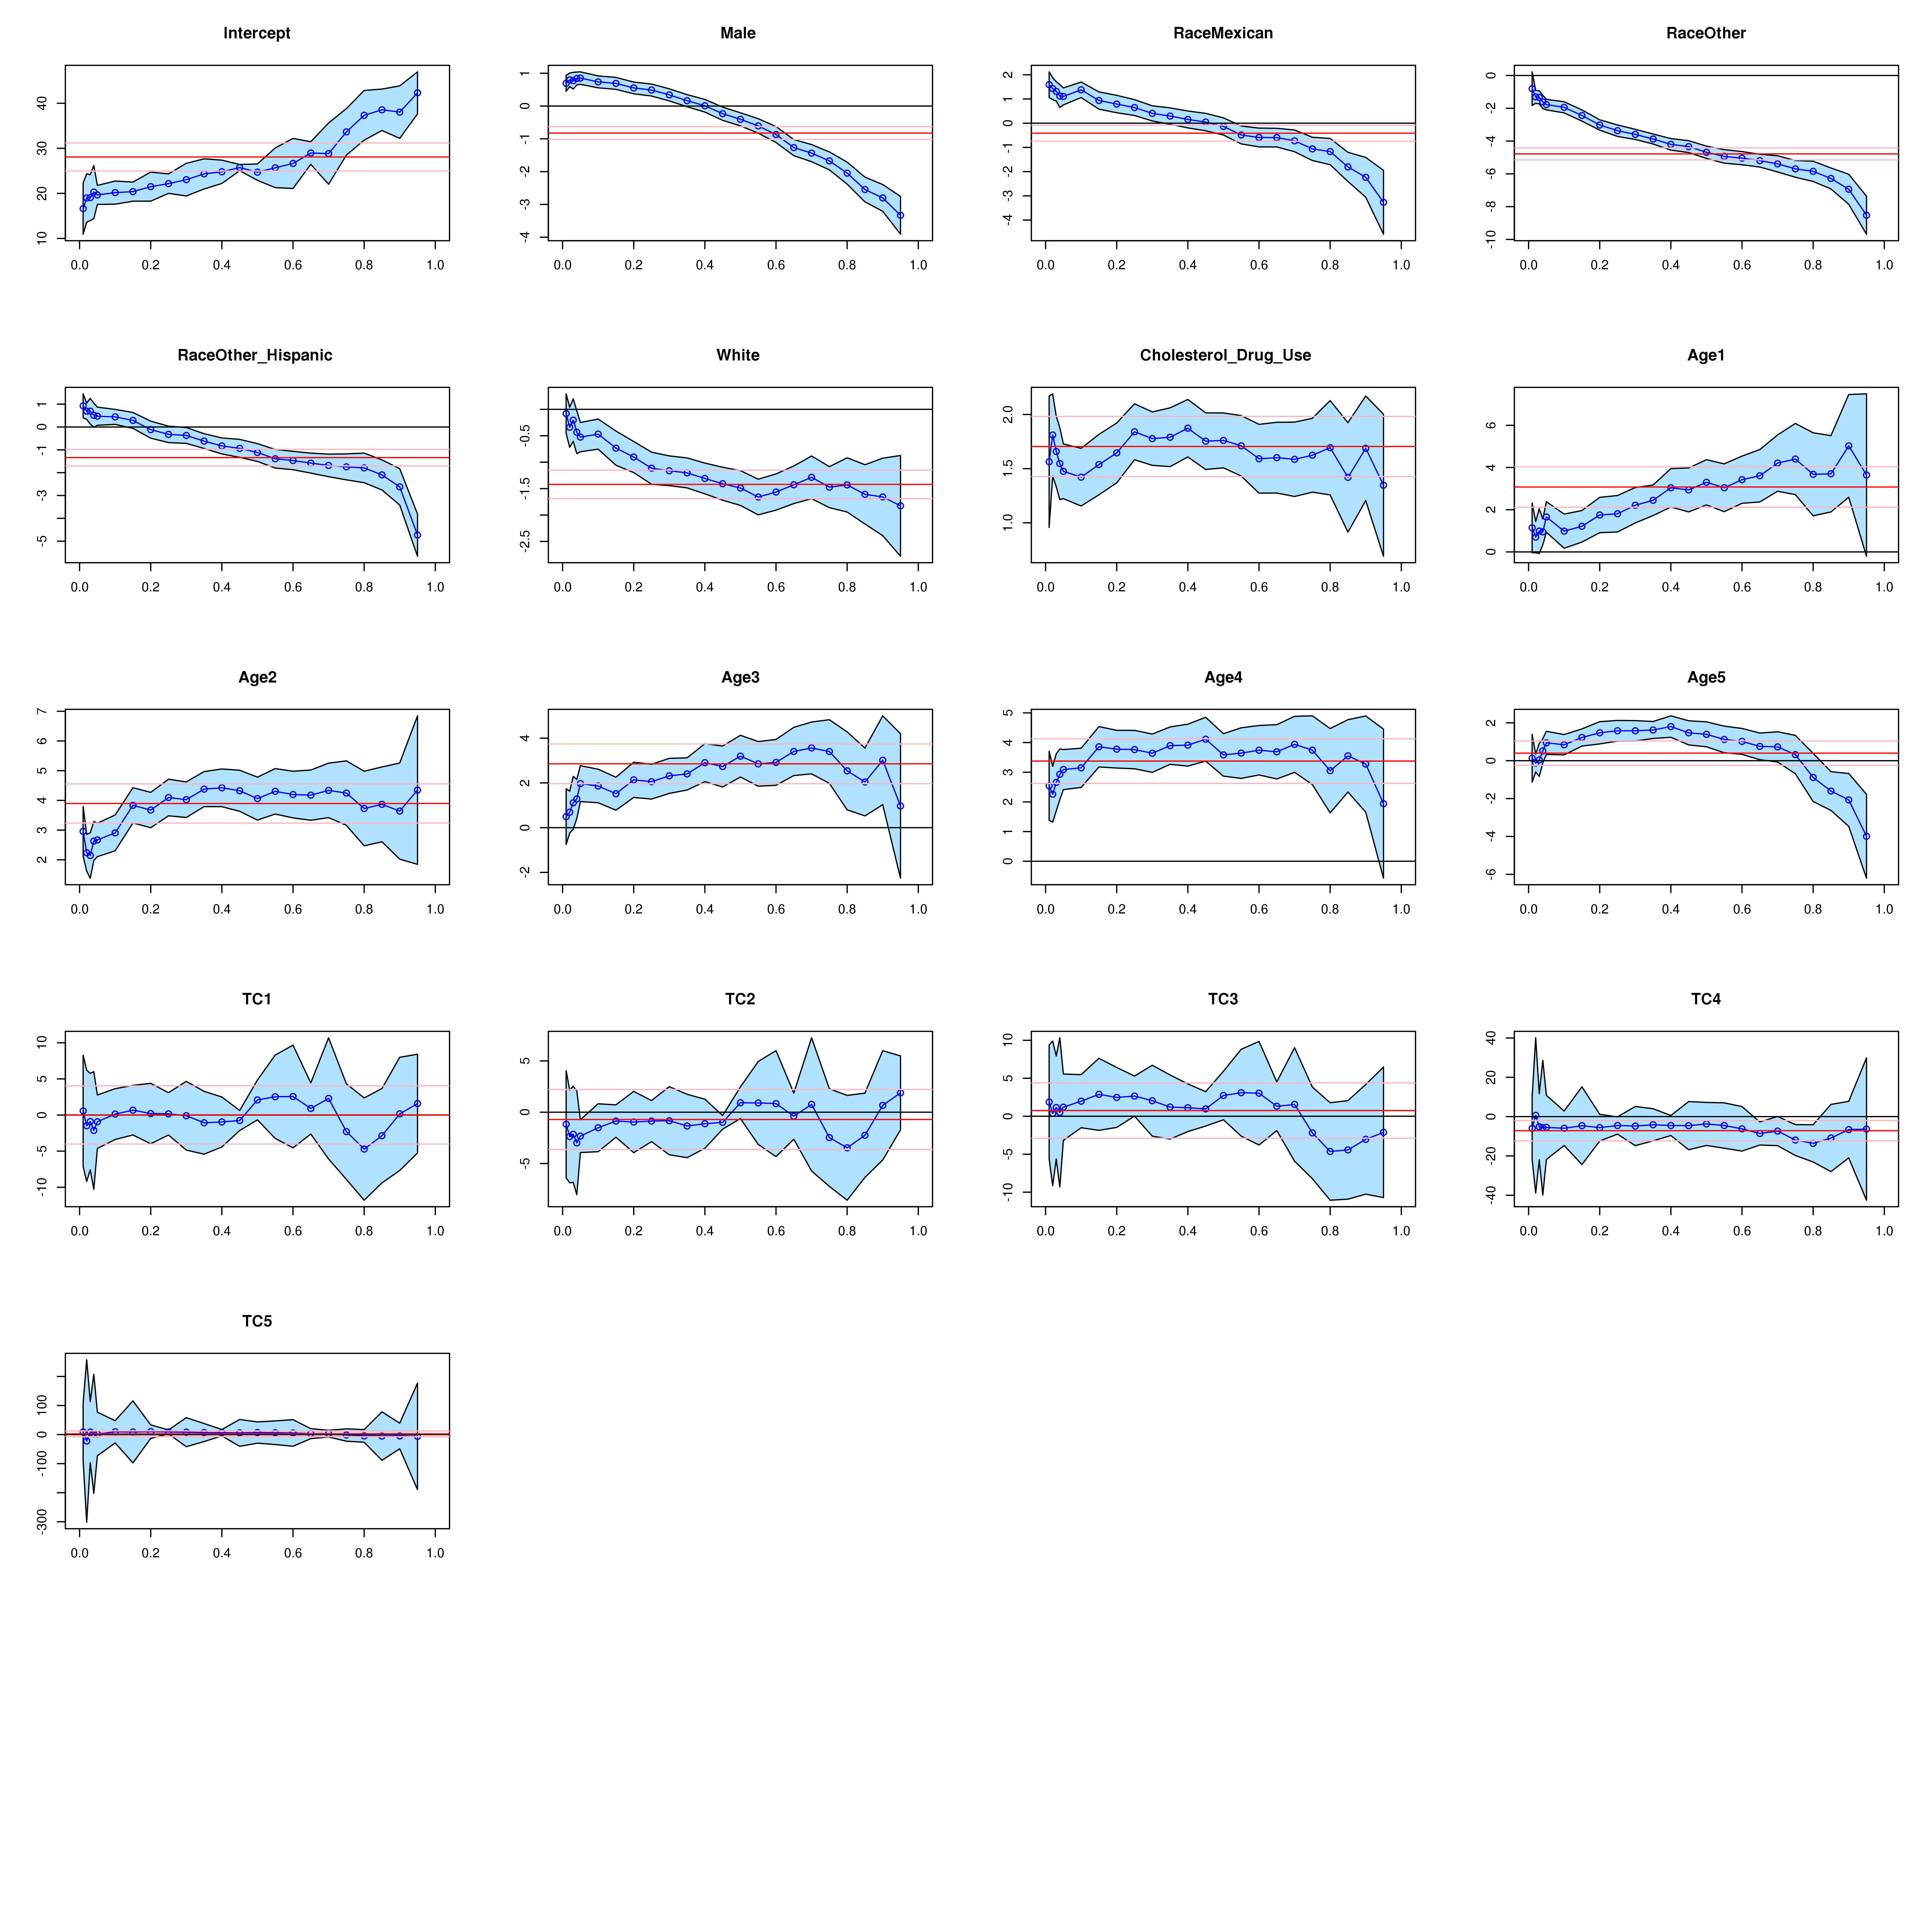
\includegraphics[width=0.8\linewidth]{C:/Users/Muhannad/Desktop/multvariat/R_codes/tonton/BMI/images/newfig11} 

}

\caption{A better figure caption}\label{fig:resu12}
\end{figure}

therefore

\begin{figure}

{\centering 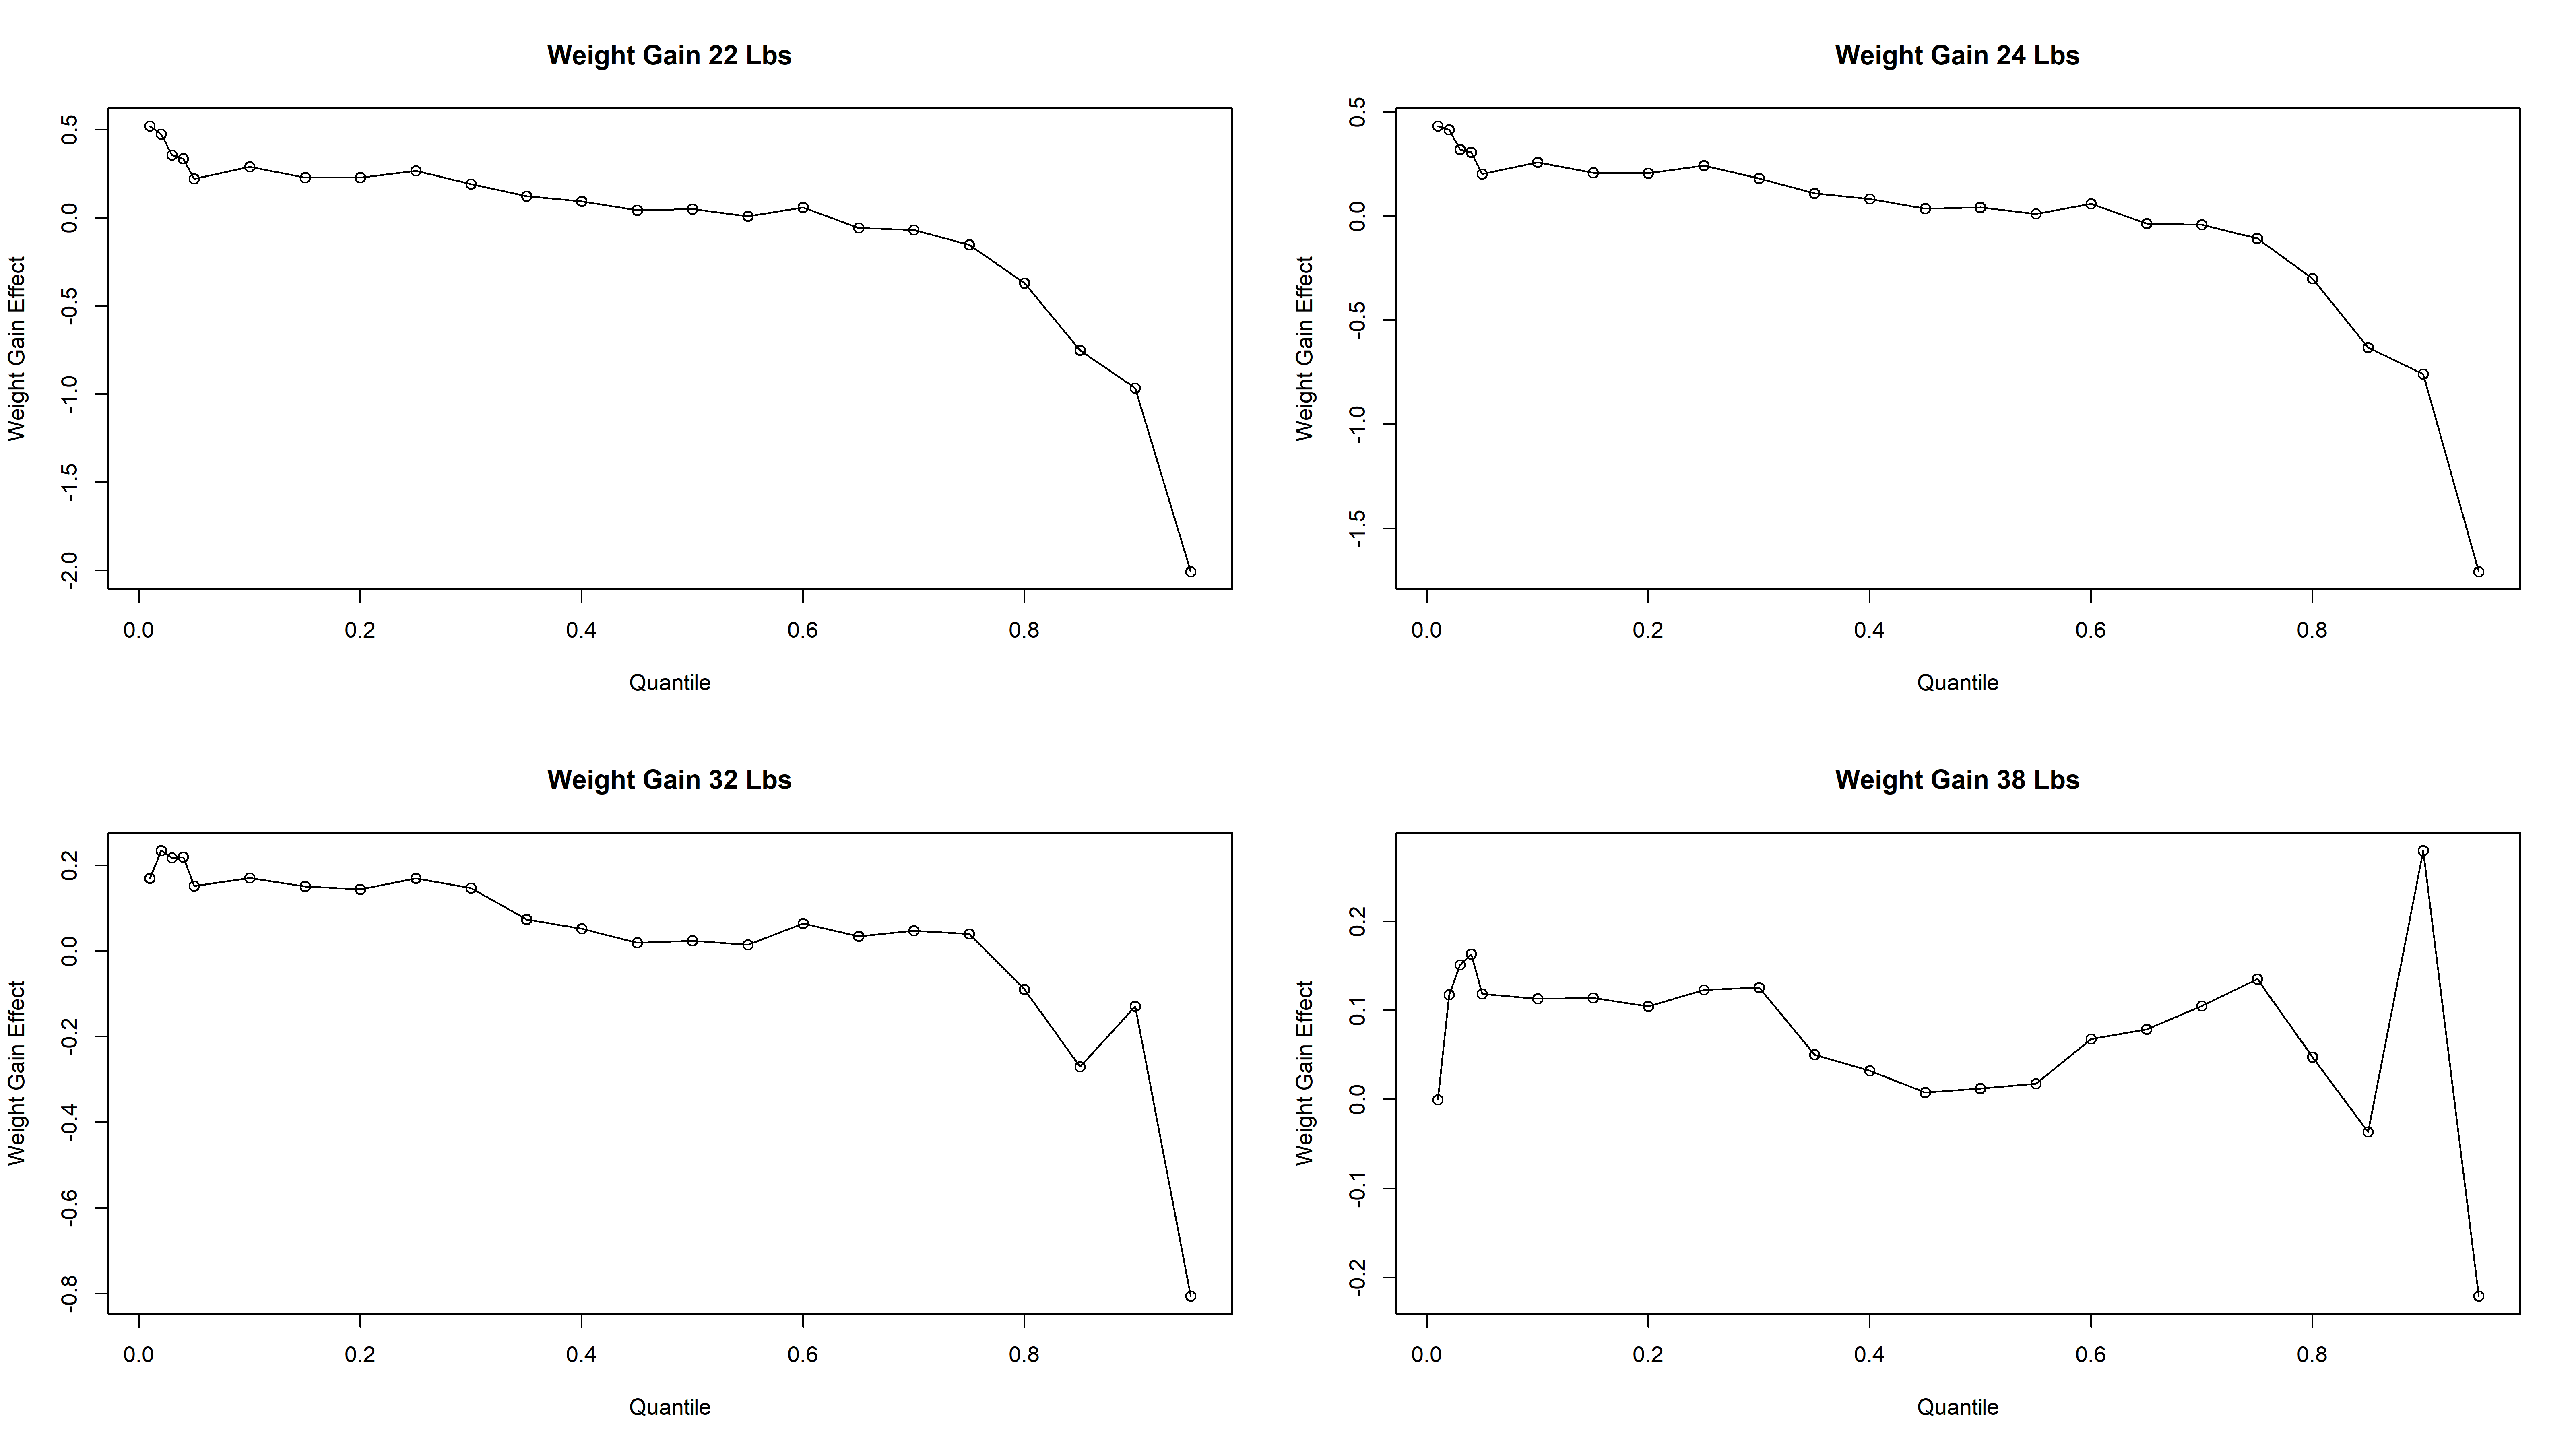
\includegraphics[width=0.8\linewidth]{C:/Users/Muhannad/Desktop/multvariat/R_codes/tonton/BMI/images/newfig2} 

}

\caption{A better figure caption}\label{fig:unnamed-chunk-3}
\end{figure}

So,

\begin{figure}

{\centering \includegraphics[width=0.8\linewidth]{C:/Users/Muhannad/Desktop/multvariat/R_codes/tonton/BMI/images/newfig22} 

}

\caption{A better figure caption}\label{fig:unnamed-chunk-4}
\end{figure}

Age effect modeled as a quadratic factor. The age effect is linear in
general, see Figure \ref{fig:resu3}. The slope for the left quantile is
lower than the slope of the right quantile. This can be interpreted as
age effect tends to increase over the entire range of conditional
distribution of glucose in faster rate for the higher quantile than in
the left quantile.In other word, diabetes population have higher rate of
change with respect to age if compared to non diabetes population. It
was found that there is a significantly correlation between glucose and
age(Tsaousis 2014).

The relation between total cholesterol and fasting glucose has been
studied in (Tsaousis 2014),(Chang et al. 2011). They found that there is
a positive correlation between the two groups. However, we found that

\begin{figure}

{\centering 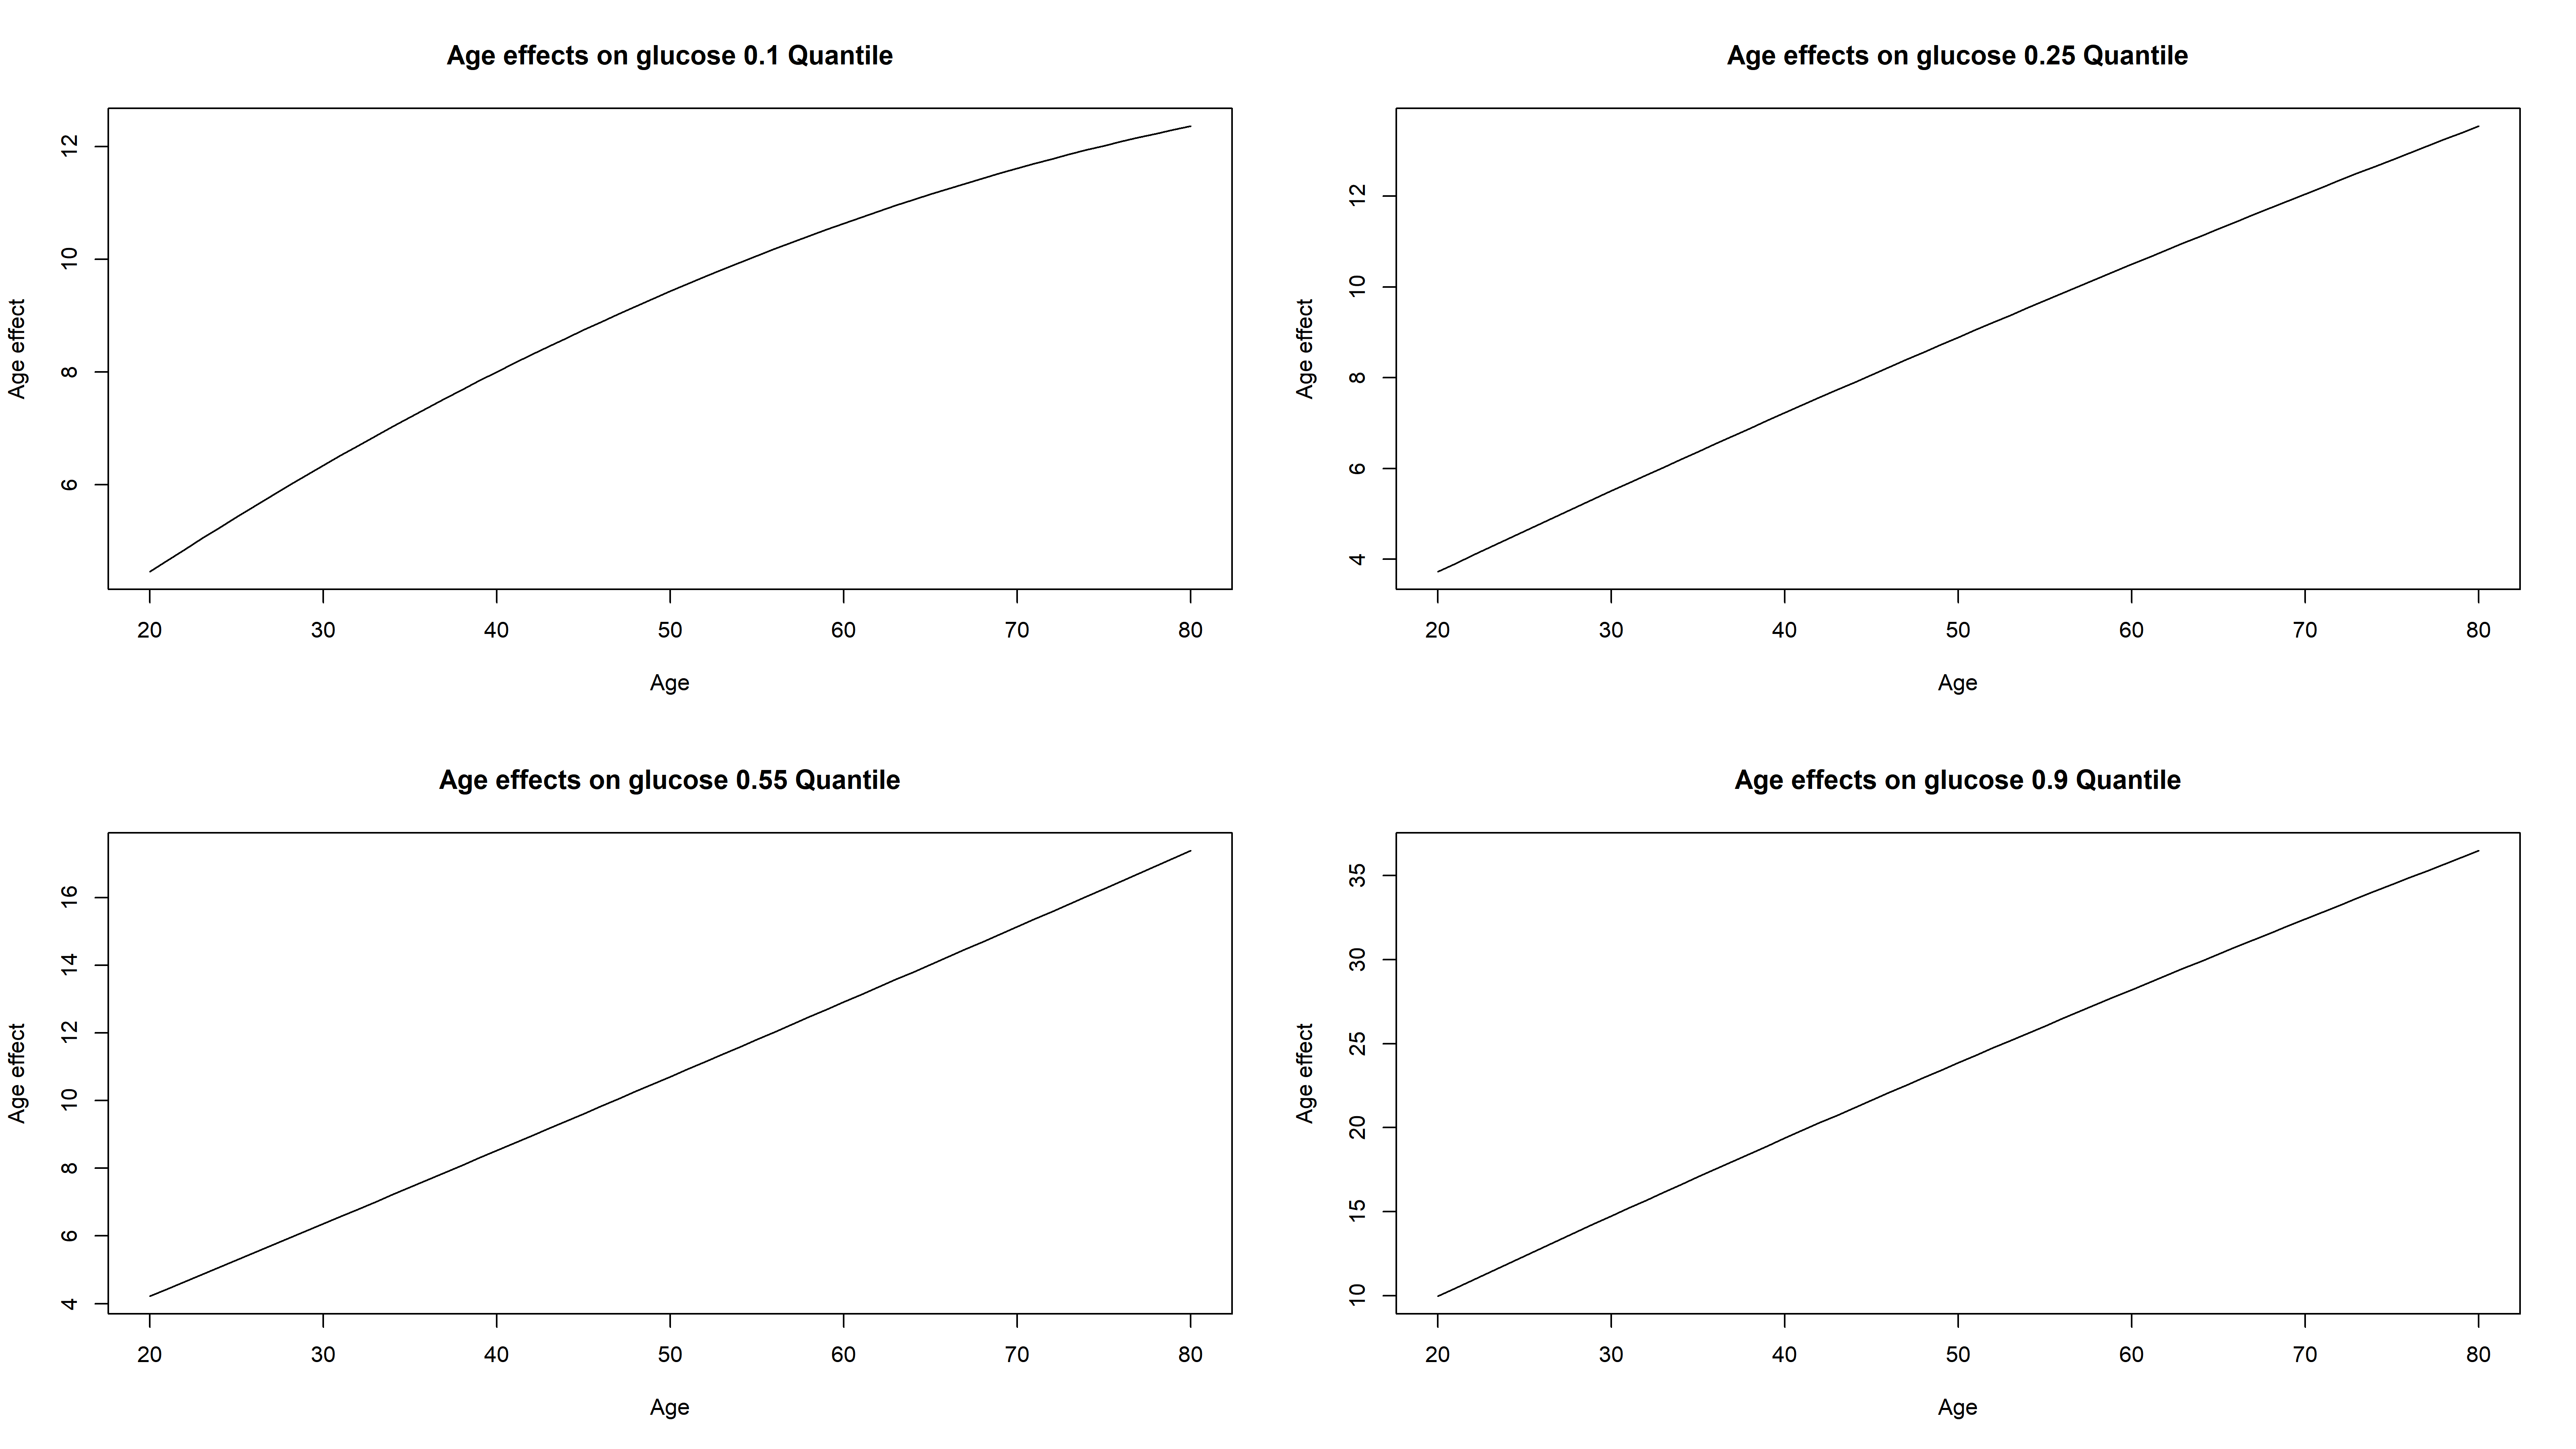
\includegraphics[width=0.8\linewidth]{C:/Users/Muhannad/Desktop/multvariat/R_codes/tonton/BMI/images/newfig3} 

}

\caption{Illustration of the quadratic age effect on glucose leveles for four different quantiles of the conditional glucose distribution.  The }\label{fig:resu3}
\end{figure}

So,

\begin{figure}

{\centering \includegraphics[width=0.8\linewidth]{C:/Users/Muhannad/Desktop/multvariat/R_codes/tonton/BMI/images/newfig33} 

}

\caption{Illustration of the quadratic age effect on glucose leveles for four different quantiles of the conditional glucose distribution.  The }\label{fig:resu33}
\end{figure}

Quadratic effect of total cholesterol on the conditional distribution of
glucose is convex. At the lower tail, decreasing glucose level by
somewhat around 1.4 up to around 180 Cholesterol level. Then, started to
increase glucose levels after TC beyond 180. At higher quantile, the
reverse in the cholesterol effects is shifted to higher cholesterol
levels which around 200, Figure \ref{fig:resu4}. The relation between
total cholesterol and fasting glucose has been studied in (Tsaousis
2014),(Chang et al. 2011). They found that there is a positive
correlation between the two groups on average.

\begin{figure}

{\centering 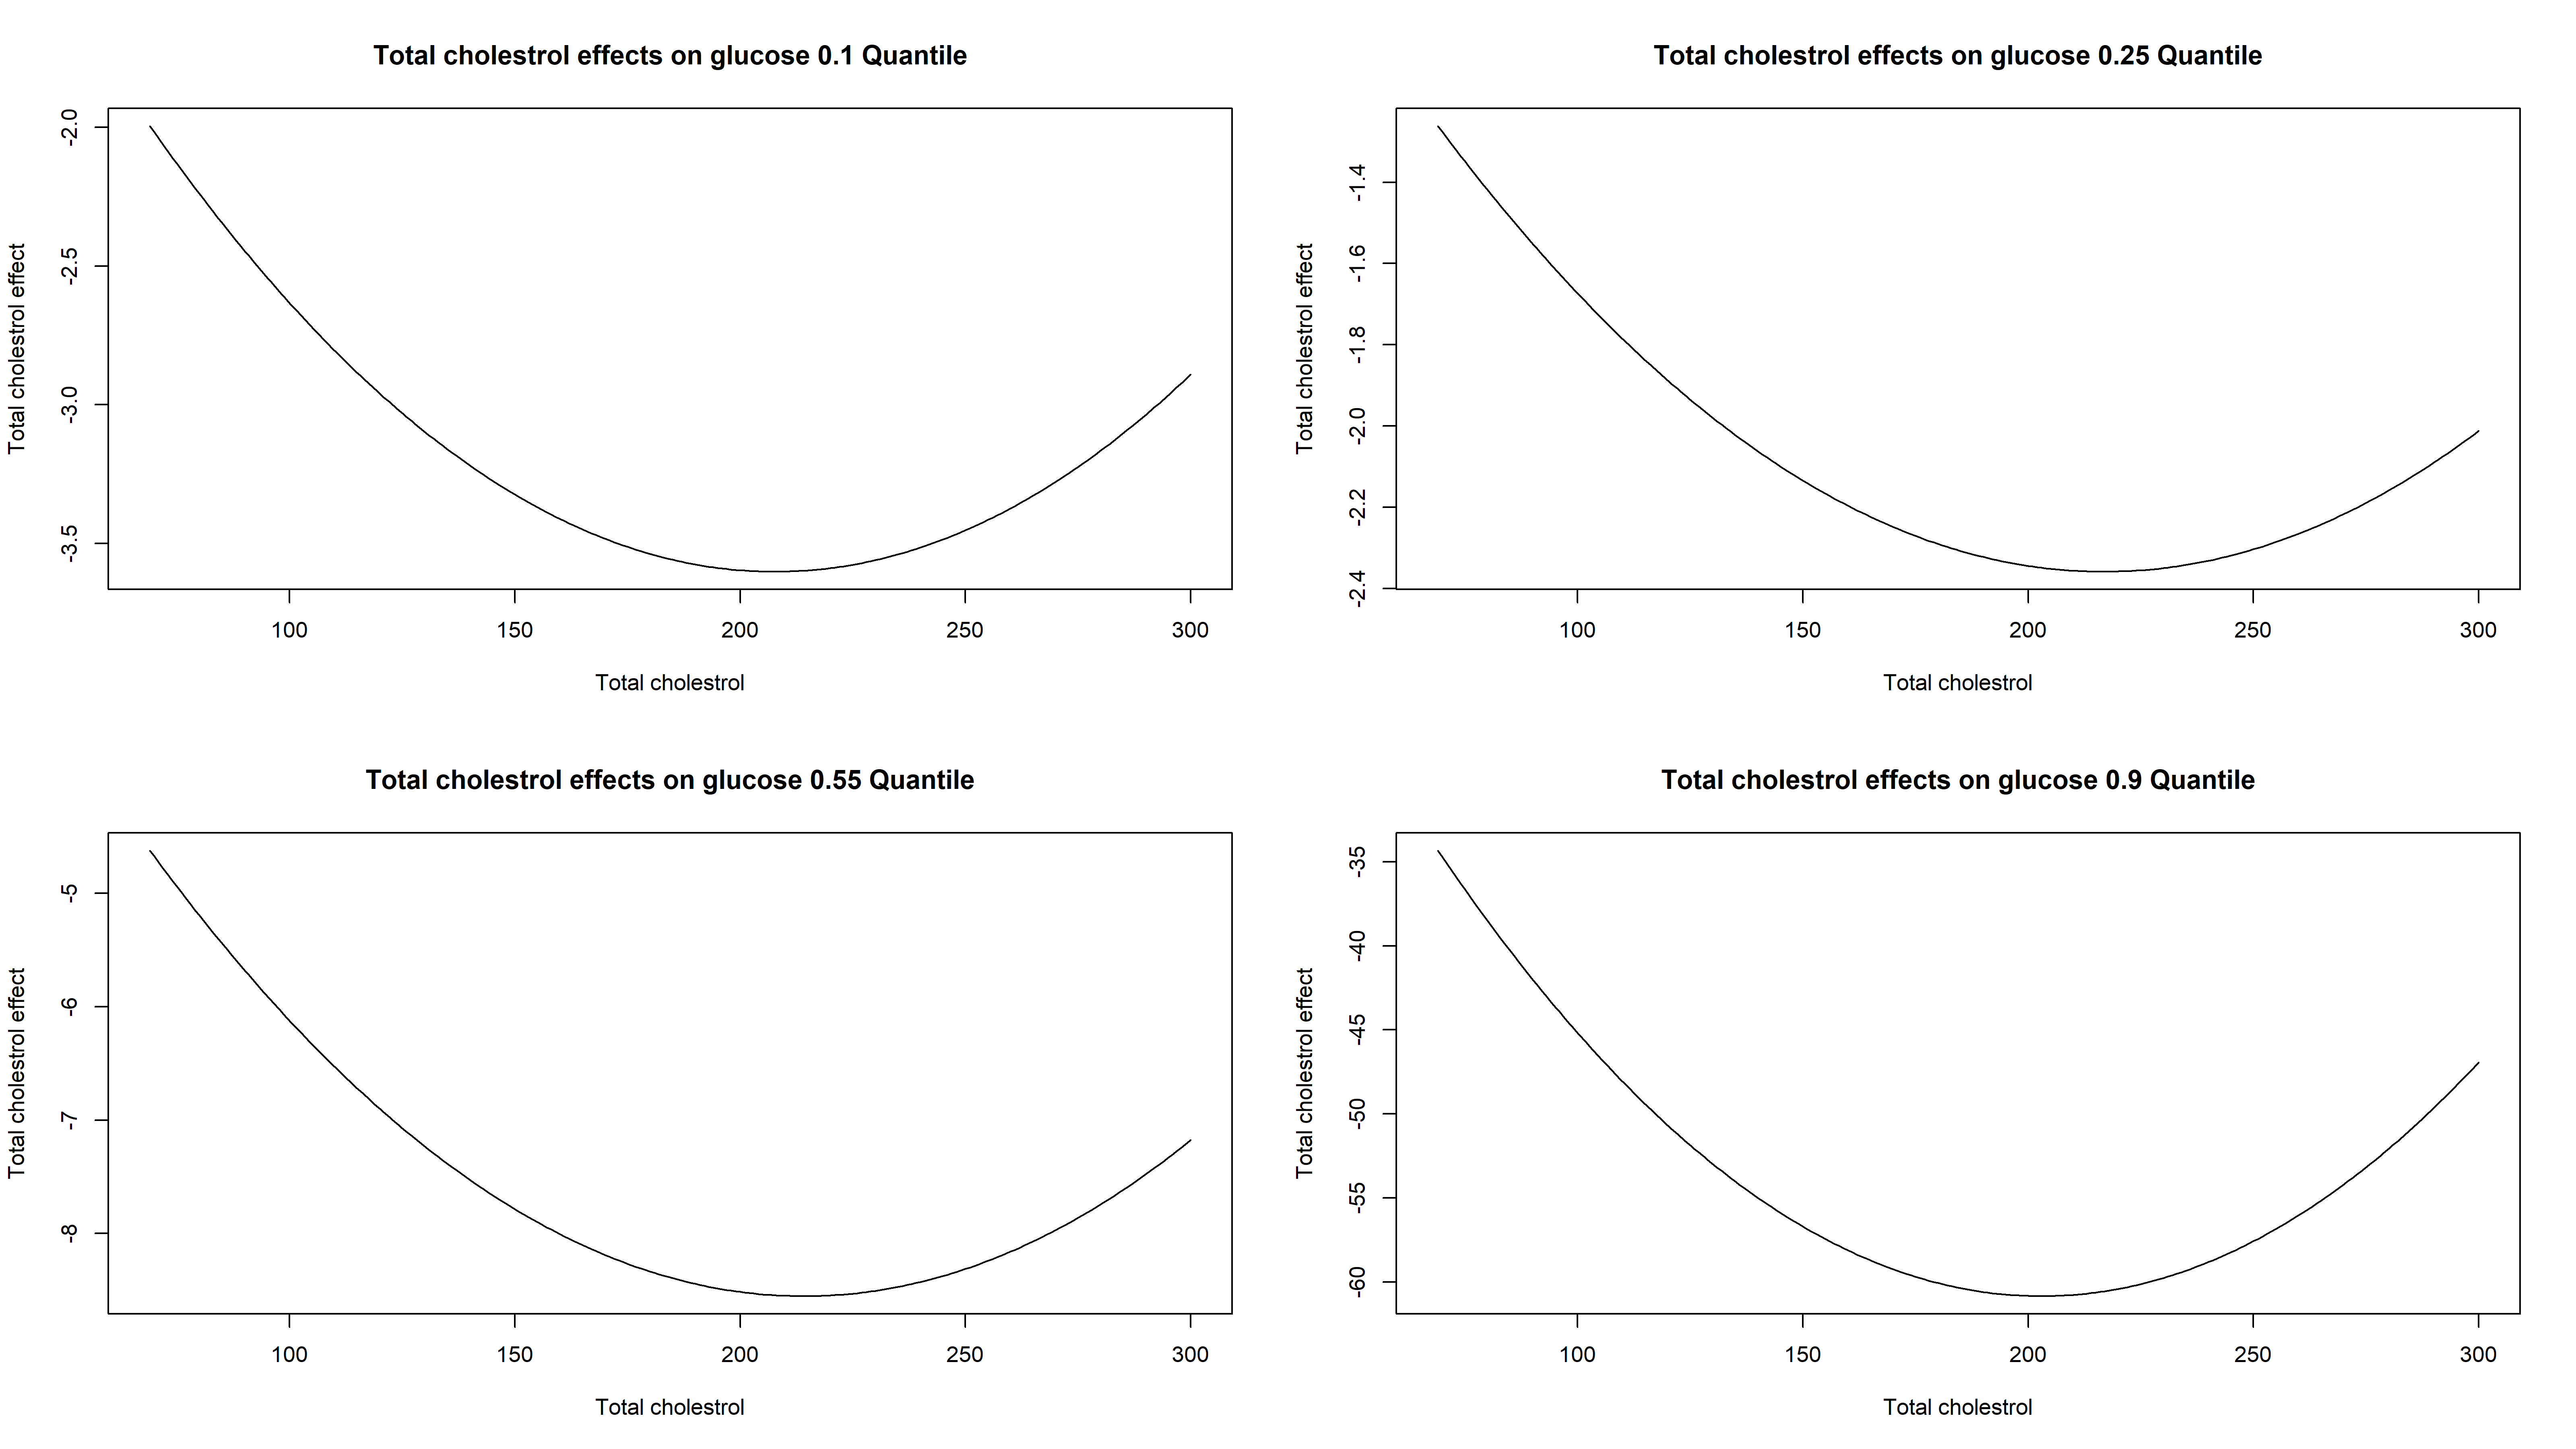
\includegraphics[width=0.8\linewidth]{C:/Users/Muhannad/Desktop/multvariat/R_codes/tonton/BMI/images/newfig4} 

}

\caption{Illustration of the quadratic cholestrol effect on glucose leveles for four different quantiles of the conditional glucose distribution.  The }\label{fig:resu4}
\end{figure}

So,

\begin{figure}

{\centering \includegraphics[width=0.8\linewidth]{C:/Users/Muhannad/Desktop/multvariat/R_codes/tonton/BMI/images/newfig44} 

}

\caption{Illustration of the quadratic cholestrol effect on glucose leveles for four different quantiles of the conditional glucose distribution.  The }\label{fig:resu44}
\end{figure}

So,

\section{Conclusion}

Multivariate quantile regression is used to study effects of different
variables on fasting glucose level. Our study showed that people who
have TC levels around 190 mg/dL have lowest fasting glucose levels for
the lowest quantile, for the second quantile optimal cholesterol level
is around 220mg/dL, and for the upper quantile the optimal cholesterol
level is around 200 mg/dL. Moreover, Statin effects on glucose at lower
quantile is very small if compared to upper quantile. \newpage
\section{References}

\hypertarget{refs}{}
\hypertarget{ref-balkau2004prediction}{}
Balkau, Beverley, Gang Hu, Qing Qiao, Jaakko Tuomilehto, Knut
Borch-Johnsen, K Pyorala, DECODE Study Group, European Diabetes
Epidemiology Group, and others. 2004. ``Prediction of the Risk of
Cardiovascular Mortality Using a Score That Includes Glucose as a Risk
Factor. the Decode Study.'' \emph{Diabetologia} 47 (12). Springer
Science \& Business Media: 2118.

\hypertarget{ref-castro2016}{}
Castro, M Regina, Gyorgy Simon, Stephen S Cha, Barbara P Yawn, L Joseph
Melton, and Pedro J Caraballo. 2016. ``Statin Use, Diabetes Incidence
and Overall Mortality in Normoglycemic and Impaired Fasting Glucose
Patients.'' \emph{Journal of General Internal Medicine} 31 (5).
Springer: 502--8.

\hypertarget{ref-chang2011}{}
Chang, Jin-Biou, Nain-Feng Chu, Jhu-Ting Syu, An-Tsz Hsieh, and Yi-Ren
Hung. 2011. ``Advanced Glycation End Products (Ages) in Relation to
Atherosclerotic Lipid Profiles in Middle-Aged and Elderly Diabetic
Patients.'' \emph{Lipids in Health and Disease} 10 (1). Springer: 228.

\hypertarget{ref-NHANES}{}
Disease Control, Centers for, and Prevention (CDC). 2018. ``National
Health and Nutrition Examination Survey Data (Nhanes.''

\hypertarget{ref-hay2017gbd}{}
Hay, Simon I, Sudha P Jayaraman, Alejandra G Contreras Manzano, Anoushka
Millear, Laura Kemmer, Brent Bell, Juan Jesus Carrero, et al. 2017.
``GBD 2015 Risk Factors Collaborators. Global, Regional, and National
Comparative Risk Assessment of 79 Behavioural, Environmental and
Occupational, and Metabolic Risks or Clusters of Risks, 1990-2015: A
Systematic Analysis for the Global Burden of Disease Study 2015 (Vol
388, Pg 1659, 2016).'' \emph{Lancet} 389 (10064). ELSEVIER SCIENCE INC
360 PARK AVE SOUTH, NEW YORK, NY 10010-1710 USA: E1--E1.

\hypertarget{ref-koenker2005}{}
Koenker, Roger. 2005. ``Quantile Regression, Volume 38 of.''
\emph{Econometric Society Monographs}.

\hypertarget{ref-mozaffarian2015executive}{}
Mozaffarian, Dariush, Emelia J Benjamin, Alan S Go, Donna K Arnett,
Michael J Blaha, Mary Cushman, Sarah De Ferranti, et al. 2015.
``Executive Summary: Heart Disease and Stroke Statistics---2015 Update:
A Report from the American Heart Association.'' \emph{Circulation} 131
(4). Am Heart Assoc: 434--41.

\hypertarget{ref-ridker2012}{}
Ridker, Paul M, Aruna Pradhan, Jean G MacFadyen, Peter Libby, and Robert
J Glynn. 2012. ``Cardiovascular Benefits and Diabetes Risks of Statin
Therapy in Primary Prevention: An Analysis from the Jupiter Trial.''
\emph{The Lancet} 380 (9841). Elsevier: 565--71.

\hypertarget{ref-tsaousis2014}{}
Tsaousis, Konstantinos T. 2014. ``Blood Glucose and Cholesterol
Concentrations in a Mediterranean Rural Population of Andros Island,
Greece.'' \emph{International Journal of Preventive Medicine} 5 (11).
Wolters Kluwer--Medknow Publications: 1464.

\hypertarget{ref-yusuf2016}{}
Yusuf, Salim, Jackie Bosch, Gilles Dagenais, Jun Zhu, Denis Xavier,
Lisheng Liu, Prem Pais, et al. 2016. ``Cholesterol Lowering in
Intermediate-Risk Persons Without Cardiovascular Disease.'' \emph{New
England Journal of Medicine} 374 (21). Mass Medical Soc: 2021--31.

\hypertarget{ref-yusuf2004effect}{}
Yusuf, Salim, Steven Hawken, Stephanie Ôunpuu, Tony Dans, Alvaro Avezum,
Fernando Lanas, Matthew McQueen, et al. 2004. ``Effect of Potentially
Modifiable Risk Factors Associated with Myocardial Infarction in 52
Countries (the Interheart Study): Case-Control Study.'' \emph{The
Lancet} 364 (9438). Elsevier: 937--52.

\end{document}
